\documentclass[12pt, titlepage]{article}

\usepackage{fullpage}
\usepackage[round]{natbib}
\usepackage{multirow}
\usepackage{booktabs}
\usepackage{tabularx}
\usepackage{graphicx}
\usepackage{float}
\usepackage{hyperref}
\hypersetup{
    colorlinks,
    citecolor=blue,
    filecolor=black,
    linkcolor=red,
    urlcolor=blue
}

\input{../../Comments}
%% Common Parts

\newcommand{\progname}{Chess Connect} % PUT YOUR PROGRAM NAME HERE
\newcommand{\authname}{Team \#4,
\\ Alexander Van Kralingen
\\ Arshdeep Aujla
\\ Jonathan Cels
\\ Joshua Chapman
\\ Rupinder Nagra} % AUTHOR NAMES without MacIDs 

\usepackage{hyperref}
    \hypersetup{colorlinks=true, linkcolor=blue, citecolor=blue, filecolor=blue,
                urlcolor=blue, unicode=false}
    \urlstyle{same}

\newcommand{\projectoverview}{

The Chess Connect project allows two users to play a game of chess on a physical board with the information being transmitted to an online web application over Bluetooth.
Currently, there is no way for players to seamlessly switch between playing on a physical board and playing online, but Chess Connect intends to change this by creating a central platform that will provide flexibility and remove barriers for new players looking to learn the game.

}

\newcounter{acnum}
\newcommand{\actheacnum}{AC\theacnum}
\newcommand{\acref}[1]{AC\ref{#1}}

\newcounter{ucnum}
\newcommand{\uctheucnum}{UC\theucnum}
\newcommand{\uref}[1]{UC\ref{#1}}

\newcounter{mnum}
\newcommand{\mthemnum}{M\themnum}
\newcommand{\mref}[1]{M\ref{#1}}

\begin{document}

\title{Module Guide for \progname{}} 
\author{\authname}
<<<<<<< HEAD
\author{\authname}
=======
>>>>>>> Documentation/DD
\date{\today}

\maketitle

\pagenumbering{roman}

\section{Revision History}

\addcontentsline{toc}{section}{Table of Revisions}
\section*{Table of Revisions}
\begin{table}[hp]
\caption{Revision History} \label{TblRevisionHistory}
\begin{tabularx}{\textwidth}{llX}
\toprule
\textbf{Date} & \textbf{Developer(s)} & \textbf{Change}\\
\midrule
<<<<<<< HEAD
1/17/2023 & 1.0 & Detailed Modules used by Arduino Mega 2560\\
2023-01-16 & Jonathan Cels, Rupinder Nagra & Web Application Modules\\
2023-01-18 & Jonathan Cels, Rupinder Nagra & Finalized Web Application Modules\\
=======
2023-01-16 & Jonathan Cels, Rupinder Nagra & Web Application Modules\\
2023-01-17 & Alexander Van Kralingen & Detailed Modules used by Arduino Mega 2560\\
2023-01-18 & Jonathan Cels, Rupinder Nagra & Finalized Web Application Modules\\
2023-01-18 & Rupinder Nagra & Introduction, Anticipated and Unlikely Changes, Connection Between Requirements and Design, Use Hierarchy Between Modules\\
2023-01-18 & Alexander Van Kralingen & Modules, Anticipated and Unlikely Changes, Connection Between Requirements and Design, Module Hierarchy\\

>>>>>>> Documentation/DD
\bottomrule
\end{tabularx}
\end{table}

\newpage

\section{Reference Material}

This section records information for easy reference.

\subsection{Abbreviations and Acronyms}

\renewcommand{\arraystretch}{1.2}
\begin{tabular}{l l} 
  \toprule		
  \textbf{symbol} & \textbf{description}\\
  \midrule 
  AC & Anticipated Change\\
  M & Module \\
  MG & Module Guide \\
  MIS & Module Interface Specification \\
  OS & Operating System \\
  R & Requirement\\
  UC & Unlikely Change \\
  \cite{FEN} & Forsyth-Edwards Notation\\
  \bottomrule
\end{tabular}\\

\newpage

\tableofcontents

\listoftables

\listoffigures

\newpage

\pagenumbering{arabic}

\section{Introduction}

\subsection{Overview}

The Chess Connect project allows two users to play a game of chess on a physical board with the information being transmitted to an online web application over Bluetooth.
Currently, there is no way for players to seamlessly switch between playing on a physical board and playing online, but Chess Connect intends to change this by creating a central platform that will provide flexibility and remove barriers for new players looking to learn the game.

\subsection{Context}

This document is the Module Guide (MG), which is created after the Software Requirements Specification (SRS). 
The purpose of the Software Requirements Specification document is to present a description of the software system to be developed, including the functional and non-functional requirements for the project. The following MG has a different purpose, where it is instead providing a modular decomposition of the system, showing the modular structure of the application. The MG also describes how the requirements in the SRS are met with the modular structure that is described.
Along with the MG, it is also necessary to create a Module Interface Specification (MIS) explaining the semantics and syntax of each module. Examples of such semantics and syntax includes the access routines, state variables, inputs/outputs, and exceptions of the modules. This document will further expand on the information provided in the MG.

\subsection{Design Principles}

Information Hiding and Encapsulation are some of the design principles being used to build a modular structure of our application. The project should also assess the software metric of coupling and cohesion. Ideally, the project has high cohesion, and a low degree of coupling.
Information Hiding is the process of hiding the details of an object or function. This process disassociates the calling code from the internal workings of the object or function being called. This makes it possible to change the hidden portions without having to also change the calling code. Encapsulation is a design principle that makes it easier to enforce information hiding. Encapsulation simply hides the states of an object of a class by preventing direct access to it. 
A high cohesion signifies that the methods and data within a module are closely related. Low coupling means that there is a low degree of interdependence between the modules of the system. 


\subsection{Document Structure}
	The document structure is organised as follows:
\begin{itemize}

\item Section 4 lists Anticipated and Unlikely Changes to the system's implementation. This list is used for the Traceability Matrices later in the document.

\item Section 5 presents the Module Hierarchy, listing all the modules and their hierarchy by levels. 

\item Section 6 describes the Connection Between Requirements and Design, which details how the software requirements are related to the modules. 

\item Section 7 describes the Module Decomposition, detailing the module secrets, services, and implementations. 

\item Section 8 provides the Traceability Matrices. The first matrix connects the functional and nonfunctional requirements to the modules. The second matrix connects anticipated changes from Section 2 to the modules.

\item Section 9 presents the Uses Hierarchy diagram for the application. The model shows the uses relations between modules.

\end{itemize}	

\section{Anticipated and Unlikely Changes} \label{SecChange}

This section lists possible changes to the system. According to the likeliness
of the change, the possible changes are classified into two
categories. Anticipated changes are listed in Section \ref{SecAchange}, and
unlikely changes are listed in Section \ref{SecUchange}.

\subsection{Anticipated Changes} \label{SecAchange}

\begin{description}
  \item[\refstepcounter{acnum} \actheacnum \label{acVerification}:] The format in which the data is passed from the hardware to the web application.
  \item[\refstepcounter{acnum} \actheacnum \label{acBoardState}:] The implementation of the data structure that stores the game board state.
  \item[\refstepcounter{acnum} \actheacnum \label{acFontAndPieces}:] User options to change the font and board size.
  \item[\refstepcounter{acnum} \actheacnum \label{acGUI}:] The GUI and interface design.
  \item[\refstepcounter{acnum} \actheacnum \label{acTimers}:] The amount of time for a move to be reflected on the web application.
\item[\refstepcounter{acnum} \actheacnum \label{acHES}:] The pin configuration for Hall-effect sensors
\item[\refstepcounter{acnum} \actheacnum \label{acLED}:] The pin configuration for LEDs
\item[\refstepcounter{acnum} \actheacnum \label{acTGS}:] Transition logic between the various game states
\item[\refstepcounter{acnum} \actheacnum \label{acHUA}:] Handling different user actions
\end{description}

\subsection{Unlikely Changes} \label{SecUchange}

\begin{description}
  \item[\refstepcounter{ucnum} \uctheucnum] The user option to play against another user online.
  \item[\refstepcounter{ucnum} \uctheucnum] The interface functionality of the system.
  \item[\refstepcounter{ucnum} \uctheucnum] The rules and values related to the game itself.
  \item[\refstepcounter{ucnum} \uctheucnum] The purpose of the system to allow users to play a game of chess against an opponent.
\item[\refstepcounter{ucnum} \uctheucnum \label{ucVML}:] Valid chess move logic.
\item[\refstepcounter{ucnum} \uctheucnum \label{ucDTD}:] Data type definition locations may be shifted between different modules.
\end{description}

\section{Module Hierarchy} \label{SecMH}

This section provides an overview of the module design. Modules are summarized
in a hierarchy decomposed by secrets in Table \ref{TblMH}. The modules listed
below, which are leaves in the hierarchy tree, are the modules that will
actually be implemented.

\begin{description}
\item [\refstepcounter{mnum} \mthemnum \label{mHH}:] Hardware-Hiding Module
\item [\refstepcounter{mnum} \mthemnum \label{mAC}:] Arduino Controler Module
\item [\refstepcounter{mnum} \mthemnum \label{mAM}:] Arduino Module
\item [\refstepcounter{mnum} \mthemnum \label{mPI}:] Piece Identification Module
\item [\refstepcounter{mnum} \mthemnum \label{mCB}:] Chess Board Module
\item [\refstepcounter{mnum} \mthemnum \label{mCM}:] Communication Module
\item [\refstepcounter{mnum} \mthemnum \label{mSS}:] Software Serial Module
\item [\refstepcounter{mnum} \mthemnum \label{mInput}:] Web Application Input Module
\item [\refstepcounter{mnum} \mthemnum \label{mDisplay}:] Display Module
\item [\refstepcounter{mnum} \mthemnum \label{mOutput}:] Web Application Output Module
\item [\refstepcounter{mnum} \mthemnum \label{mMode}:] User Mode Module
\item [\refstepcounter{mnum} \mthemnum \label{mBoard}:] Board Module
\item [\refstepcounter{mnum} \mthemnum \label{mGame}:] Web Application Game State Module
\item [\refstepcounter{mnum} \mthemnum \label{mEngine}:] Engine Module
\end{description}

The Hardware-Hiding module is implemented by the microcontroller as firmware that controls all of the hardware components. This is implemented by the kernel to also run embedded software loaded onto the controller. The Arduino and SoftwareSerial modules are present in the Arduino framework and will not be recreated for this project.


\begin{table}[h!]
\centering
\begin{tabular}{p{0.3\textwidth} p{0.6\textwidth}}
\toprule
\textbf{Level 1} & \textbf{Level 2}\\
\midrule

\multirow{3}{0.3\textwidth}{Hardware Hiding Module}
& Arduino Controller Module \\ 
& Arduino Module \\
& Software Serial Module \\
\midrule

\multirow{5}{0.3\textwidth}{Behaviour-Hiding Module} 
& Web Application Input Module\\
& Display Module\\
& Web Application Output Module\\
& Piece Identification Module \\
& Communication Module\\
& Teensy Input from Mega Module\\
& Teensy Input Bluetooth from Web App Module\\
& Teensy Output Bluetooth from Web App Module\\
\midrule

\multirow{5}{0.3\textwidth}{Software Decision Module} 
& User Mode Module\\
& Board Module\\
& Web Application Game State Module\\
& Engine Module\\
& Chess Board Module\\
\bottomrule

\end{tabular}
\caption{Module Hierarchy}
\label{TblMH}
\end{table}

\section{Connection Between Requirements and Design} \label{SecConnection}

The design satisfies the system requirements developed in the SRS. The Web Application 
Input module will handle all interactions from the inputs provided by the user, such as the 
FEN String, the user mode, and whether the game has terminated. The Display module outputs 
the visual component of the interface, and this module will cover all requirements that have a 
component of the user directly interacting with the system. The Web Application Board and Game 
State modules cover the board setup and positions along with checking the end game conditions 
such as checkmate and stalemate. The look and feel requirements are satisfied by the input and 
output modules as they define the core areas of user interaction. The usability and humanity 
requirements are again satisfied by the input and output modules which define the user interaction. 
Performance requirements are to be satisfied by the combination of all modules, but the key modules 
that impact performance are software decision hiding modules. The operational and environmental 
requirements, and the maintainability and support requirements are achieved by all modules. This 
is because all modules are designed to be operational for the environment (the server and client) 
and maintained for a set time (end of semester). Security and legal requirements are covered by 
the entirety of the system. This is because the accessibility of the repository and the JavaScript 
standard in use affects all modules.

\section{Module Decomposition} \label{SecMD}

\subsection{Hardware Hiding Modules (\mref{mHH})}

\begin{description}
\item[Secrets:]The data structure and algorithm used to implement the virtual
  hardware.
\item[Services:]Serves as a virtual hardware used by the rest of the
  system. This module provides the interface between the hardware and the
  software. So, the system can use it to display outputs or to accept inputs.
\item[Implemented By:] OS
\end{description}

\subsubsection{Arduino Controller Module (\mref{mAC})}
\begin{description}
\item[Secrets:] The logic for changing game state and reading user actions.
\item[Services:] Reads inputs from sensors and writes to outputs to turn on/off LED's. Main overarching module that runs and controls all other modules to coordinate the logic and messages with the game state.
\item[Implemented By:] \progname (Arduino Mega 2560 Rev3 Controller)
\end{description}

\subsubsection{Arduino Module (\mref{mAM})}
\begin{description}
\item[Secrets:] The Arduino API that allows access to the Hardware Abstraction Layer (HAL).
\item[Services:] Provides an interface to the hardware through pin assignments and hardware ID's.
\item[Implemented By:] Arduino.h library
\end{description}

\subsubsection{Piece Identification Module (\mref{mPI})}
\begin{description}
\item[Secrets:] The values read by the Hall-effect sensors that are translated into the Piece data type.
\item[Services:] Translates sensor values into pieces and positions on the chess board. Provides Piece identification data types to the rest of the program.
\item[Implemented By:] \progname (c++, Arduino)
\end{description}

\subsubsection{Chess Board Module (\mref{mCB})}
\begin{description}
\item[Secrets:] Contained within this module are: 
  \begin{itemize}
    \item the valid move logic for chess pieces; 
    \item The translation of the piece configuration on the chess board into a \href{https://en.wikipedia.org/wiki/Forsyth%E2%80%93Edwards_Notation}{FEN string} \item Checking for checkmate
  \end{itemize}
\item[Services:] Handles all of the logic used in the game of chess. This module processes commands recieved from the Web Application and Teensy Controller into actions to be implemented within the game and gives feedback related to valid moves and the game/board state.
\item[Implemented By:] \progname (c++, Arduino)
\end{description}

\subsubsection{Communication Module (\mref{mCM})}
\begin{description}
\item[Secrets:] Message encoding string used to send board state, game mode and resignation signal. Message decoding string to interpret best moves, the check/mate/stalemate warning and commands from the Teensy controller.
\item[Services:] Reads and writes to the communication pins, processes and sends commands to various parts of the embedded software.
\item[Implemented By:] \progname (c++, Arduino, Bluetooth)
\end{description}

\subsubsection{Software Serial Module (\mref{mSS})}
\begin{description}
\item[Secrets:] The methods in which the data is encoded, flags used to acknowledge connection, successful data transmission, incoming signal, etc.
\item[Services:] The Arduino API that allows for sending and receiving various data types through serial communication.
\item[Implemented By:] SoftwareSerial.h library
\end{description}

\subsection{Behaviour-Hiding Modules}
    \subsubsection{Web Application Input Module (\mref{mInput})}
    \begin{description}
    \item[Secrets:] Input data.
    \item[Services:] Takes in input data of current board state to provide to other modules.
    \item[Implemented By:] \progname\ (Node.js libraries, Bluetooth)
    \end{description}
    
    \subsubsection{Display Module \mref{mDisplay}} 
    \begin{description}
    \item[Secrets:] Graphics output data.
    \item[Services:] Allows users to view the current board configuration of the system.
    \item[Implemented By:] \progname\ (React.js framework)
    \end{description}

    \subsubsection{Web Application Output Module \mref{mOutput}} 
    \begin{description}
    \item[Secrets:] None.
    \item[Services:] Takes game state and engine moves, encodes the data, and transmits it.
    \item[Implemented By:] \progname\ (React.js framework, Bluetooth)
    \end{description}

\subsection{Software Decision Modules}
    \subsubsection{User Mode Module \mref{mMode}}
    \begin{description}
    \item[Secrets:] User mode logic and data.
    \item[Services:] Handles switching between user modes and communicating with mode-specific modules.
    \item[Implemented By:] \progname\ (React.js framework)
    \end{description}

    \subsubsection{Web Application Board Module \mref{mBoard}}
    \begin{description}
    \item[Secrets:] Board data.
    \item[Services:] Stores and modifies board state information.
    \item[Implemented By:] \progname\ (React.js framework)
    \end{description}

    \subsubsection{Web Application Game State Module \mref{mGame}}
    \begin{description}
    \item[Secrets:] Game state and data.
    \item[Services:] Handles checking the game state (none, check, checkmate, stalemate).
    \item[Implemented By:] \progname\ (React.js framework, Node.js libraries)
    \end{description}
    
    \subsubsection{Engine Module \mref{mEngine}}
    \begin{description}
    \item[Secrets:] Chess engine moves.
    \item[Services:] Uses the board state to calculate 3 possible moves.
    \item[Implemented By:] \progname\ (Node.js libraries and Stockfish)
    \end{description}



\section{Traceability Matrix} \label{SecTM}
This section shows two traceability matrices: between the modules and the
requirements and between the modules and the anticipated changes.

% the table should use mref, the requirements should be named, use something
% like fref
\begin{table}[H]
\centering
\begin{tabular}{p{0.4\textwidth} p{0.4\textwidth}}
\toprule
\textbf{Req.} & \textbf{Modules}\\
\midrule
R1 & \mref{mHH}, \mref{mInput}, \mref{mParams}, \mref{mControl}\\
R2 & \mref{mInput}, \mref{mParams}\\
R3 & \mref{mVerify}\\
R4 & \mref{mOutput}, \mref{mControl}\\
R5 & \mref{mOutput}, \mref{mODEs}, \mref{mControl}, \mref{mSeqDS}, \mref{mSolver}, \mref{mPlot}\\
R6 & \mref{mOutput}, \mref{mODEs}, \mref{mControl}, \mref{mSeqDS}, \mref{mSolver}, \mref{mPlot}\\
R7 & \mref{mOutput}, \mref{mEnergy}, \mref{mControl}, \mref{mSeqDS}, \mref{mPlot}\\
R8 & \mref{mOutput}, \mref{mEnergy}, \mref{mControl}, \mref{mSeqDS}, \mref{mPlot}\\
R9 & \mref{mVerifyOut}\\
R10 & \mref{mOutput}, \mref{mODEs}, \mref{mControl}\\
R11 & \mref{mOutput}, \mref{mODEs}, \mref{mEnergy}, \mref{mControl}\\
R12 & \mref{TeensyToMegaRx} \mref{TeensyToWaRx} \mref{TeensyToWaTx}\\

\bottomrule
\end{tabular}
\caption{Trace Between Requirements and Modules}
\label{TblRT}
\end{table}

\begin{table}[H]
\centering
\begin{tabular}{p{0.2\textwidth} p{0.6\textwidth}}
\toprule
\textbf{AC} & \textbf{Modules}\\
\midrule
\acref{acHES} & \mref{mAC}\\
\acref{acLED} & \mref{mAC}\\
\acref{acTGS} & \mref{mAC}, \mref{mCB}\\
\acref{acHUA} & \mref{mAC}, \mref{mCB}, \mref{mCM}\\
\bottomrule
\end{tabular}
\caption{Trace Between Anticipated Changes and Modules}
\label{TblACT}
\end{table}

\section{Use Hierarchy Between Modules} \label{SecUse}

\begin{figure}[H]
\centering
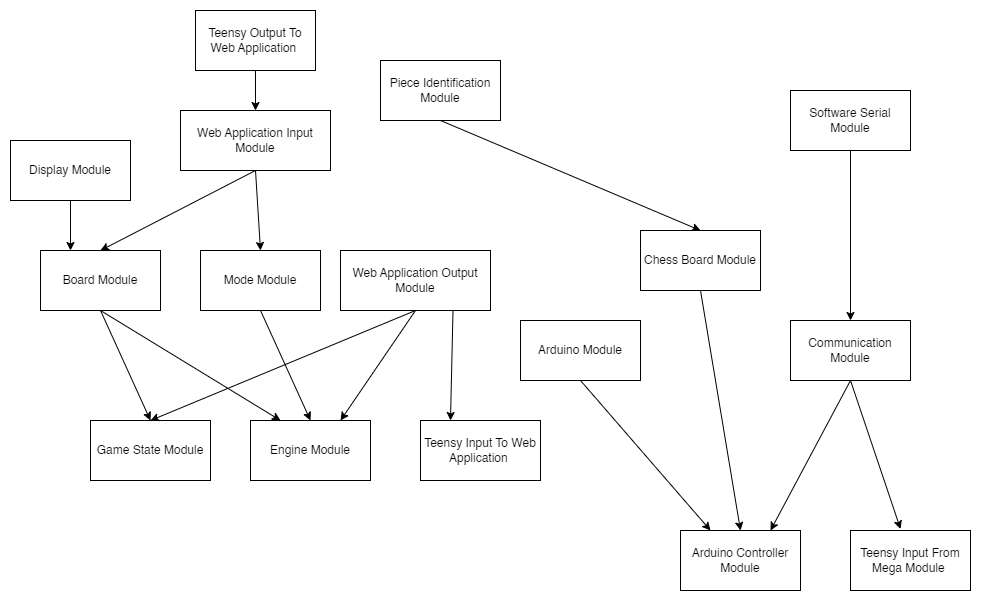
\includegraphics[width=0.7\textwidth]{ModuleHierarchy.png}
\caption{Use hierarchy among modules}
\label{FigUH}
\end{figure}

%\section*{References}

\bibliographystyle {plainnat}
\bibliography{../../../refs/References}

\end{document}